\documentclass[a4paper]{book}
\usepackage[czech]{babel}
\usepackage[IL2]{fontenc}
\usepackage[utf8]{inputenc}
\usepackage{pstricks}
\usepackage{amsmath}
\usepackage{graphicx}
\usepackage{pdfpages}
\usepackage{mathrsfs}

%\includeonly{mood_chap5}

\setlength{\unitlength}{1.0mm}
\sloppy

\begin{document}

\newtheorem{definition}{Definice}[chapter]
\newtheorem{theorem}{Věta}[chapter]
\newtheorem{proof}{Důkaz}[chapter]
\newtheorem{example}{Příklad}[chapter]
\newtheorem{proposition}{Tvrzení}[chapter]
\newtheorem{corollary}{Tvrzení}[chapter]
\newtheorem{fallacy}{Omyl}[chapter]

\hyphenation{prav-dě-po-dob-nost prav-dě-po-dob-nost-ní} 

\title{Kopule - souhrn vybraných článků}
\author{Michal Mackanič}
\date{2014}
\maketitle

\tableofcontents

\chapter{Úvod}

\section{Definice kopule}

Uvažujme náhodné veličiny $X_1$ a $X_2$. Předpokládejme, že známe hodnotu náhodné proměnné $X_1$, a že na základě této informace máme odhadnout hodnotu náhodné proměnné $X_2$. Pro zodpovězení této otázky je klíčová znalost vztahu mezi náhodnými veličinami $X_1$ a $X_2$.

Pokud mezi oběma náhodnými veličinami neexistuje žádný vztah, tj. jedná-li se o nezávislé náhodné veličiny, pak informace o hodnotě náhodné veličiny $X_1$ nám neříká nic o hodnotě náhodné veličiny $X_2$. Naopak, platí-li $X_1 = X_2$, pak, známe-li $X_1$, známe také $X_2$. Vedle těchto dvou extrémní případů, existuje také řada jiných možností, např. $X_1 \le X_2$.

Pro hlubší analýzu budeme potřebovat nástroj pro popis závislostí dvou náhodných veličin. Každá jednotlivá náhodná veličina je popsána svou kumulativní distribuční funkcí (cdf - cumulative distribution function) definovanou jako $F_i(x) := P(X_i \le x)$. Nicméně tyto marginální distribuční funkce nám neříkají nic o společném ``chování'' uvažovaných náhodných veličin. K tomu je zapotřebí tzv. sdružená distribuční funkce. V případě nezávislosti je tato funkce definována jako
\begin{equation*}
P(X_1 \le x_1, X_2 \le x_2) = F_1(x_1)F_2(x_2)
\end{equation*}
Pro úplný popis $X_1$ a $X_2$ tedy potřebujeme dvě ``ingredience'' - marginální distribuční funkci a vyjádření závislosti uvažovaných náhodných veličin. Otázkou zůstává, zda-li je možné rozložit libovolnou sdruženou distribuční funkci na marginální distribuční funkce a funkci, která vyjadřuje jejich závislost. Dle Sklarovy věty to možné je. Řešení problému spočívá v transformaci hodnot jednotlivých náhodných veličin na kvantily a následnému vyjádření jejich ``závislosti'' pomocí tzv. kopula funkce\footnote{Pro ilustraci uvažujme akcie $A$ a $B$, pro které máme dispozici vývoj cen pro určité časové období. Nejprve pro každou jednotlivou akcii odhadneme na základě pozorovaných cen její distribuční funkci. Následně s pomocí distribuční funkce transformujeme každou cenu na odpovídající kvantil $a_t$ resp. $b_t$. Každému datu $t$ tak bude přiřazen kvantilový bod $(a_t, b_t)$. Posledním krokem je pak odhad kopula funkce, která pokud možno co nejlépe popíše ``chování'' těchto bodů z hlediska pravděpodobnosti jejich realizace.}.

\begin{definition}[Kopule]
Kopule je vícerozměrná kumulativní distribuční funkce, jejíž jednotlivá marginální rozdělení sledují rovnoměrné rozdělení $U[0, 1]$. Kopule je tedy funkcí, která mapuje z $d$-rozměrného prostoru $[0, 1]^d$ do jednorozměrného prostoru $[0, 1]$, neboli $C : [0, 1]^d : \rightarrow [0, 1]$.
\end{definition}
V následujícím textu budeme pro kopuli používat notaci $C(u) = C(u_1, ..., u_d)$. Skutečnost, že kopule $C$ je distribuční funkcí, má za následek následující.
\begin{itemize}
\item Protože je distribuční funkce z definice rostoucí funkcí, je kopula funkce $C(u_1, ..., u_d)$ taktéž rostoucí v každé náhodné veličině $u_i$.
\item Marginální rozdělení náhodné veličiny $u_i$ lze získat dosazením $u_i = 1$ pro všechna $j \neq i$. Toto marginální rozdělení sleduje rovnoměrné rozdělení $U[0, 1]$.
\begin{equation*}
C(1, ..., 1, u_i, 1, ..., 1) = u_i
\end{equation*}
\item Pro $a_i < b_i$ musí být pravděpodobnost $P(U_1 \in [a_1, b_1], ..., U_d \in [a_d, b_d])$ nezáporná, což vede k tzv. trojúhelníkové nerovnosti
\begin{equation*}
\sum_{i_1 = 1}^2 \dots \sum_{i_d = 1}^2 (-1)^{i_1 + \dots + i_d}C(u_{1, i_1}, ..., u_{d, i_d}) \ge 0,
\end{equation*}
kde $u_{j,1} = a_j$ a $a_{j,2} = b_j$.
\end{itemize}
Každá funkce, která splňuje výše uvedené podmínky, je kopula funkcí. Dále platí, že je-li $C$ $d$-rozměrnou kopula funkcí, pak $C(1, u_1, ..., u_{d-1})$ je $d-1$ rozměrnou kopula funkcí. Proto se řada teoretických otázek může omezit pouze na problematiku dvourozměrné kopula funkce.

Jak již bylo řečeno, hlavní myšlenkou kopula funkce je ``rozložit'' vícerozměrné náhodné rozdělení na mariginální distribuční funkce a funkci vyjadřující závislost kvantilů jednotlivých náhodných veličin. Klíčem k tomu je tzv. kvantilová transformace, která se často používá při simulování náhodných veličin. Pro distribuční funkci $F$ definujeme obecnou inverzní funkci jako
\begin{equation*}
F^{\leftarrow}(y) := \inf\{x: F(x) \ge y\}
\end{equation*}
\begin{proposition}[Inverzní kumulativní distribuční funkce]
Jestliže náhodná veličina $U$ sleduje uniformní rozdělení $U[0, 1]$ a $F$ je kumulativní distribuční funkcí, pak
\begin{equation}
P(F^{\rightarrow}(U) \le x) = F(x)
\end{equation}
Obráceně, jestliže náhodná veličina $Y$ má spojitou distribuční funkci $F$, pak platí
\begin{equation}
F(Y) \sim U[0, 1]
\end{equation}
\end{proposition}

\begin{figure}[htp]
\centering
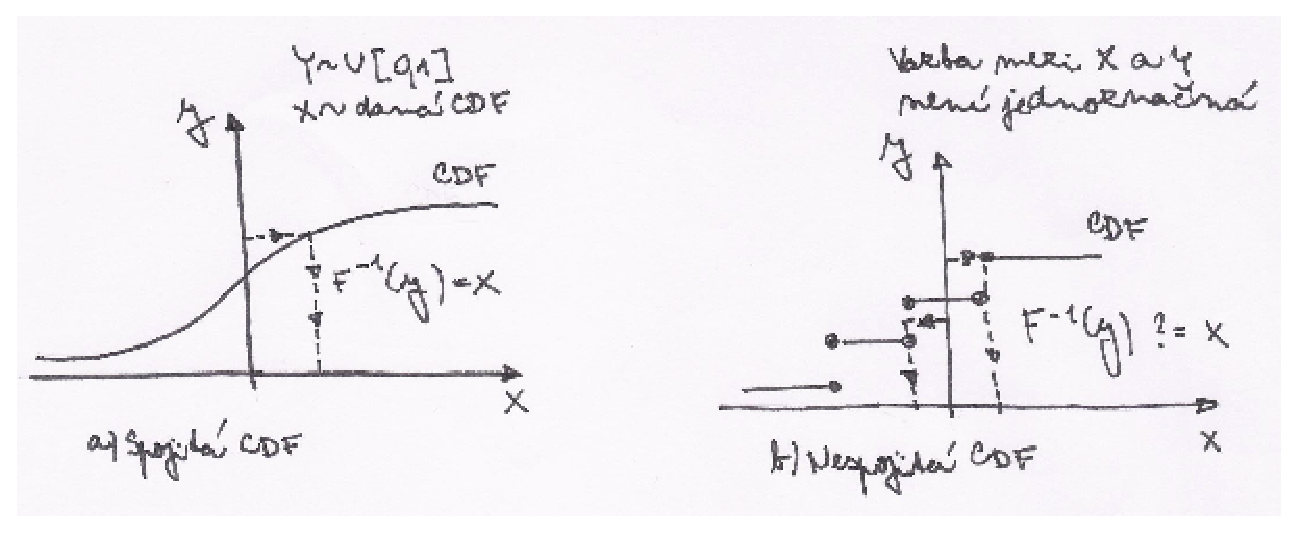
\includegraphics[scale = 0.5]{pictures/inv_cdf.eps}
\caption{Inverze kumulativní distribuční funkce}
\label{inv_cdf}
\end{figure} 

\subsection{Sklarova věta}

Libovolná distribuční funkce definovaná nad $R^d$ v sobě implicitně zahrnuje kopula funkci. Toto tvrzení platí také naopak. Jestliže ``spojíme'' kopula funkci a marginální cdf, získáme vícerozměrné rozdělení. Toto tvrzení vyplývá z následující věty.

\begin{theorem}[Sklarova věta]
Uvažujme $d$-rozměrnou distribuční funkci $F$ s marginálními distribučními funkcemi $F_1, ..., F_d$. Pak existuje kopula funkce taková, že
\begin{equation}
F(x_1, ..., x_d) = C\big(F_1(x_1), ..., F_d(x_d)\big)
\end{equation}
pro všechna $x_i$ v $(-\infty, \infty)$, $i = 1, ..., d$. Jestliže je $F_i$ spojitá pro všechna $i = 1, ..., d$, pak je $C$ jedinečné. V opačném případě je $C$ jedinečné pouze na $Ran(F_1) \times \cdots \times Ran(F_d)$, kde $Ran(F_i)$ označuje obor hodnot distribuční funkce $F_i$\footnote{Např. pro hrací kostku je obor hodnot příslušné distribuční funkce definován jako $\{\frac{1}{6}, \frac{2}{6}, ..., \frac{6}{6}\}$.}.

Výše uvedené tvrzení platí i naopak. Uvažujme kopula funkci $C$ a jednorozměné distribuční funkce $F_1, ..., F_d$. Pak $F$ definovaná dle (1.3) je vícerozměrnou distribuční funkcí s marginálními distribučními funkcemi $F_1, ..., F_d$.
\end{theorem}
S využitím vztahu $F_i \circ F_i^{\leftarrow}(y) \ge y$ získáváme
\begin{equation}
C(u) = F\big(F_1^{\leftarrow}(u_1), ..., F_d^{\leftarrow}(u_d)\big)
\end{equation}
Zatímco (1.3) je zpravidla výchozím bodem pro simulaci, vztah (1.4) slouží spíše pro ``oddělení'' kopula funkce od vícerozměrné distribuční funkce.

\subsection{Hustota pravděpodobnosti kopule}

Dle definice je kopula funkce distribuční funkcí. Vzhledem k obtížné interpretaci kumulativní distribuční funkce se často používá hustota pravděpodobnosti (pdf - probability density function). Je však třeba zmínit, že ne všechny kopula funkce mají odpovídající hustotu pravděpodobnosti. Nicméně má-li kopula funkce diferenci požadovaného řádu, lze hustotu pravděpodobnosti vyjádřit jako
\begin{equation*}
c(u) := \frac{\partial^d C(u_1, ..., u_d)}{\partial u_1, ..., u_d}
\end{equation*}

Jestliže lze kopula funkci vyjádřenou ve tvaru (1.4) derivovat, což má za následek $F_i^{\leftarrow} = F_i^{-1}$, lze odpovídající hustotu pravděpodobnosti vyjádřit jako
\begin{equation*}
c(u) = \frac{f\big(F_1^{-1}(u_1), ..., F_d^{-1}(u_d)\big)}{f_1\big(F_1^{-1}(u_1)\big) \cdots f_d\big(F_d^{-1}(u_d)\big)}
\end{equation*}
kde $f$ označuje sdruženou hustotu pravděpodobnosti a $f_i, i = 1, ..., d$ marginální hustotu pravděpodonosti jednotlivých náhodných veličin.
\begin{proof}
S využitím pravidla pro derivaci složené funkce (chain rule)
\begin{equation*}
\frac{d f(g(x))}{dx} = \frac{df}{dg}\frac{dg}{dx} = f'(g(x))g'(x)
\end{equation*}
a skutečností $F(F^{-1}(u)) = u$ a $\frac{du}{du} = 1$, lze snadno dokázat
\begin{equation*}
\frac{dF(F^{-1}(u))}{du} = f(F^{-1}(u))\frac{dF^{-1}(u)}{du} = 1
\end{equation*}
z čehož vyplývá
\begin{equation*}
\frac{dF^{-1}(u)}{du} = \frac{1}{f(F^{-1}(u))}
\end{equation*}
Derivací dvourozměné kopule funkce ve tvaru (1.4) tak získáme
\begin{multline*}
\frac{dF\big(F_1^{-1}(u_1),F_2^{-2}(u_2)\big)}{du_1du_2} = f\big(F_1^{-1}(u_1), F_2^{-1}(u_2)\big)\frac{F_1^{-1}(u_1)}{du_1}\frac{F_2^{-1}(u_2)}{du_2}\\
= \frac{f\big(F_1^{-1}(u_1), F_2^{-1}(u_2)\big)}{f_1\big(F_1^{-1}(u_1)\big)f_2\big(F_2^{-1}(u_2)\big)}
\end{multline*}
\end{proof}

\subsection{Podmíněné rozdělení}

Uvažujme dvě uniformní náhodné veličiny $U_1$ a $U_2$. Předpokládejme, že známe kopula funkci $C$ a hodnotu náhodné veličiny $U_1$. Cílem je odvodit podmíněné rozdělení, které lze použít pro odhad náhodné veličiny $U_2$. Za předpokladu dostatečné regularity lze odvodit podmíněnou distribuční funkci.
\begin{multline*}
P(U_2 \le u_2 | U_1 = u_1) = \lim_{\delta \rightarrow 0}\frac{P(U_2 \le u_2, U \in (u_1 - \delta, u_1 + \delta])}{P(U_1 \in (u_1 - \delta, u_1 + \delta])}\\
= \lim_{\delta \rightarrow 0}\frac{C(u_1 + \delta, u_2) - C(u_1 - \delta, u_2)}{2 \delta} = \frac{\partial C(u_1, u_2)}{\partial u_1}
\end{multline*}
Podmíněné distribuční funkce lze tedy odvodit derivací kopula funkce $C$ dle $u_1$. Odpovídající podmíněnou hustotu pravděpodobnosti lze získat následnou derivací dle $u_2$.

\subsection{Hraniční hodnoty kopule}

\begin{proposition}
Uvažujme náhodné veličiny $X_1, ..., X_d$, jejichž závislost je definovaná kopula funkcí $C$. Nechť $T_i: R \rightarrow R, i = 1, ..., d$ je striktně rostoucí funkcí. Pak je závislost náhodných veličin $T_1(X_1), ..., T_d(X_d)$ definována toutéž kopula funkcí $C$. 
\end{proposition}
Jinými slovy, striktně rostoucí transformace nemění strukturu závislosti, což se na první podhled může zdát kontraintuitivní. Monotonní transformace totiž sice mění závislost mezi náhodnými veličinami, nicméně po očištění o vliv marginálních distribučních funkcí získáme shodnou strukturu závislosti definovanou kopula funkcí $C$.

Hoeffding a Fréchet nezávisle na sobě odvodili, že kopula funkce vždy leží v rámci určitých hraničních hodnot. Důvody lze nalézt při zkoumání extrémních případů závislosti.
Uvažujme dvě náhodné veličiny $U_1$ a $U_2$. Jestliže $U_1 = U_2$, pak hovoříme o tzv. komonotonických (comonotic) náhodných veličinách a jejich kopula funkce je dána vztahem
\begin{equation}
C(u_1, u_2) = P(U_1 \le u_1, U_1 \le u_2) = min(u_1, u_2)
\end{equation}
Tento typ kopule získéme vždy, když $X_2 = T(X_1)$, kde $T$ je monotonní transformace.
V případě, kdy jsou $U_1$ a $U_2$ nezávislé, je kopula funkce rovna
\begin{equation}
C(u_1, u_2) = u_1 u_2
\end{equation}
Dalším extrémní situací je $U_2 = 1 - U_1$, kdy hovoříme o tzv. kontramonotonických (countermonotonic) náhodných veličinách. Kopula funkce pro $1 - u_2 < u_1$ je
\begin{multline}
C(u_1, u_2) = P(U_1 \le u_1, U_2 \le u_2) = P(U_1 \le u_1, 1 - U_1 \le u_2)\\
= P(U_1 \le u_1, U_1 \ge 1 - u_2) = P(1 - u_2 \le U_1 \le u_1)\\
= u_1 - (1 - u_2) = u_1 + u_2 - 1
\end{multline}
Výše uvedené lze rozšířit na vícerozměrné rozdělení. Ačkoliv komonotonická kopule existuje pro libovolnou dimenzi $d$, kontramonotonická kopule existuje pouze pro $d = 2$\footnote{Uvažujme náhodné veličiny $X_1$, $X_2$ a $X_3$. Jako kontramonotonické zvolme páry $(X_1, X_2)$ a $(X_1, X_3)$. Tato volba představuje omezení pro závislost mezi $X_2$ a $X_3$. Jestliže se $X_1$ sníží, jak $X_2$ tak $X_3$ se musí zvýšit a tudíž nemohou být kontramonotonické.}, nicméně hraniční hodnoty jsou platné i pro vyšší dimenze.

\begin{theorem}[Fréchet-Hoeffdingovy hraniční hodnoty]
Uvažujme kopula funkci $C(u) = C(u_1, ..., u_d)$. Pak platí
\begin{equation*}
\max\left(\sum_{i = 1}^d u_i + 1 - d, 0 \right) \le C(u) \le \min\left(u_1, ..., u_d\right)
\end{equation*}
\end{theorem}

\begin{figure}[htp]
\centering
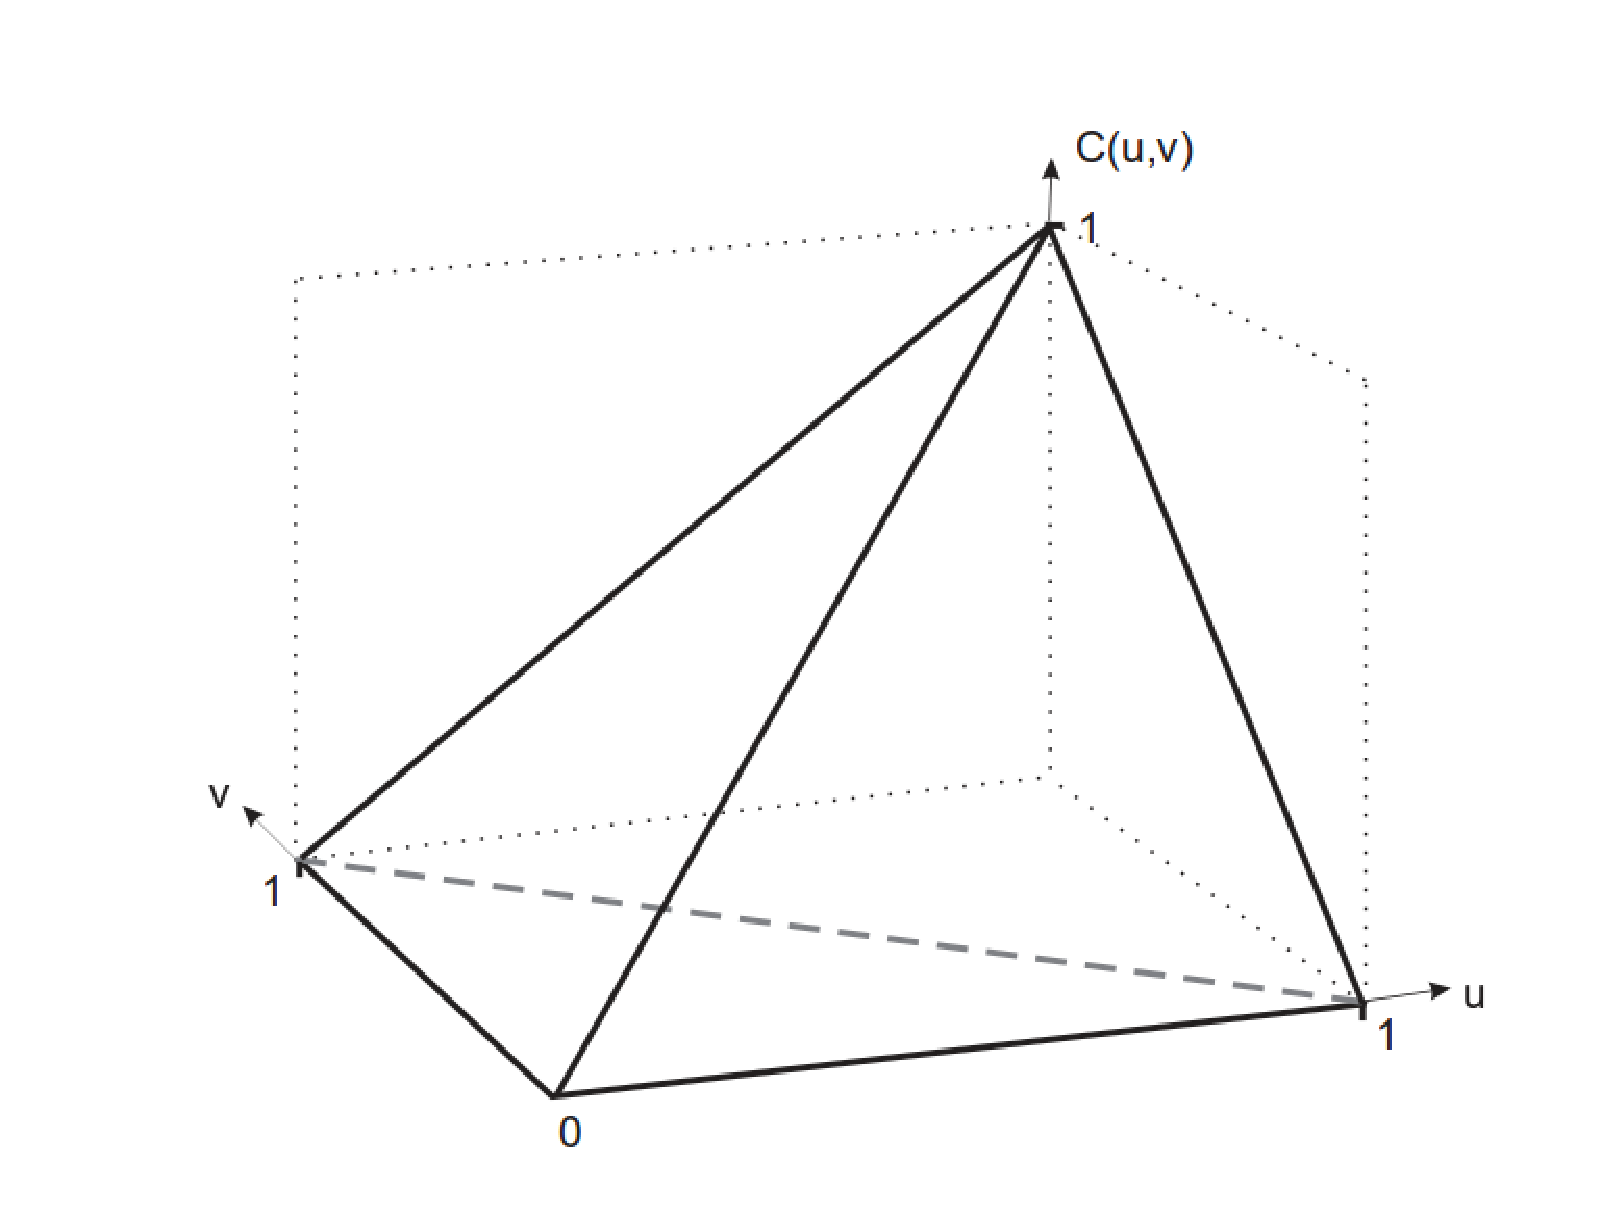
\includegraphics[scale = 0.35]{pictures/copula_boundary.eps}
\caption{Fréchet-Hoeffdingovy hraniční hodnoty - Každá kopula funkce leží uvnitř zobrazené pyramidy. Povrch daný spodní a zadní stěnou pyramidy (dolní hranice) představuje kontramonotonistickou kopula funkcí $C(u, v) = \max\{u + v -1, 0\}$. Povrch daný přední stěnou pyramidy (horní hranice) pak představuje monotonostickou kopula funkci $C(u, v) = \min(u, v)$.}
\label{copula_boundary}
\end{figure} 

\chapter{Míra závislosti}

\section{Korelace}

Korelace $\rho(X_1, X_2)$ mezi náhodnými veličinami $X_1$ a $X_2$ je definována jako
\begin{equation*}
\rho(X_1, X_2) = \frac{cov(X_1, X_2)}{\sqrt{D(X_1)D(X_2)}}
\end{equation*}
kde
\begin{equation*}
cov(X_1, X_2) = E[(X_1 - E[X1])(X_2 - E[X_2])]
\end{equation*}
Korelace vyjadřuje míru lineární závislosti a nabývá hodnot z intervalu $[-1, 1]$. Jestliže jsou $X_1$ a $X_2$ nezávislé, pak $\rho(X_1, X_2) = 0$. Opačné trvzení však neplatí - pokud je korelace rovna nula, neznamená to, že jsou $X_1$ a $X_2$ nezávislé. Pokud $|\rho(X_1, X_2)| = 1$ jsou $X_1$ a $X_2$ dokonale lineárně korelované, což znamená, že $X_2 = \alpha + \beta X_1$ téměř jistě pro některé $\alpha \in R$ a $\beta \neq 0$\footnote{V případě $\beta > 0$ hovoříme o pozitivní lineární korelaci. V případě $\beta < 0$ hovoříme o negativní lineární korelaci.}. Pro $\beta_1, \beta_2 > 0$ navíc platí
\begin{equation*}
\rho(\alpha_1 + \beta_1 X_1, \alpha_2 + \beta_2 X_2) = \rho(X_1, X_2)
\end{equation*}
což znamená, že korelace je invariantní pro striktně rostoucí lineární transformaci. Nicméně je třeba zdůraznit, že korelace není invariantní pro nelineární striktně rostoucí trasformaci $T: R \rightarrow R$. Pro dvě náhodné veličiny tedy obecně platí $\rho(T(X_1), T(X_2)) \neq rho(X_1, X_2)$.

\begin{fallacy}
Sdružená distribuční funkce je jednoznačně definována pomocí marginálních distribučních funkcí a párových korelací.
\end{fallacy}

Toto tvrzení je platné pouze v případě vícerozměrných eliptických rozdělení. Kdyby toto tvrzení bylo platné obecně, nebylo by zapotřebí konceptu kopula funkce.

\begin{example}
Uvažujme dvě náhodné veličiny představující zisk / ztrátu dvou portfolií. Předpokládejme, že obě rizika sledují standardní normální rozdělení a že jejich korelace je rovna nule. Zkonstruujme dva náhodné vektory v souladu s těmito předpoklady.

Uvažujme dvě modelové situaci. Model 1 je standardní dvourozměrné normální rozdělení $X \sim N_2(0, I_2)$. V modelu 2 nezávislá náhodná veličina $V$ s pravděpodobnostní funkcí $P(V = 1) = P(V = -1) = \frac{1}{2}$ použita při konstrukci nových náhodných veličin $(Y_1, Y_2) = (X_1, VX_1)$, kde $X_1$ je převzato z modelu 1. Marginální distribuční funkce náhodných veličin $Y_1$ a $Y_2$ sledují taktéž standardní normální rozdělení s nulovou korelací. Kopula funkce modelu 2 je
\begin{equation*}
C(u_1, u_2) = \frac{1}{2} \max(u_1 + u_2 - 1, 0) + \frac{1}{2}\min(u_1, u_2)
\end{equation*}
což je mix dvourozměrných kopula funkcí s Fréchetovou hraniční hodnotou. Náhodné velčiny $Y_1$ a $Y_2$ tedy nejsou nezávislé.
\end{example}

\begin{fallacy}
Pro libovolné jednorozměrné distribuční funkce $F_1$ a $F_2$ a libovolnou korelaci $\rho$ z intervalu $[-1, 1]$ je vždy možné zkonstruovat sdruženou distribuční funkci $F$ s marginálními distribučními funkcemi $F_1$ a $F_2$ a korelací $\rho$.
\end{fallacy}

Toto tvrzení je opět platné pouze pro eliptické pravděpodobnostní rozdělení. Tzv. dosažitelné korelace mohou tvořit podmnožinu intervalu $[-1, 1]$.

\begin{proposition}
Jestliže $(X_1, X_2)$ sleduje sdruženou distribuční funkci $F$ a marginální distribuční funkce $F_1$ a $F_2$, pak je kovariance $X_1$ a $X_1$, pokud je konečná, dána vztahem
\begin{equation}
cov(X_1, X_2) = \int_{-\infty}^{\infty} \int_{-\infty}^{\infty}(F(x_1, x_2) - F_1(x_1)F_2(x_2))dx_1 dx_2
\end{equation}
\end{proposition}

\begin{proof}
Nechť $(X_1, X_2)$ sleduje sdruženou distribuční funkci $F$ a nechť $(\tilde{X}_1, \tilde{X}_2)$ je její nezávislou kopií\footnote{Jedná se tedy o druhý pár, který sleduje sdruženou distribuční funkci $F$ a který je nezávislý na $(X_1, X_2)$.}. Platí
\begin{multline*}
E[(X_1 - \tilde{X}_1)(X_2 - \tilde{X}_2)] = E[X_1X_2 - X_1\tilde{X}_2 - \tilde{X}_1X_2 + \tilde{X}_1 \tilde{X}_2]\\
= E[X_1X_2] - E[X_1 \tilde{X}_2] + E[\tilde{X}_1 \tilde{X}_2] - E[\tilde{X}_1X_2]\\
= E[X_1X_2] - E[X_1]E[X_2] + E[X_1X_2] - E[X_1]E[X_2]\\
= 2 cov(X_1, X_2)
\end{multline*}
Nyní použijme identitu, která říká, že pro libovolné $a \in R$ a $b \in R$ platí $(a - b) = \int_{-\infty}^{\infty}(I_{\{b \le x\}} - I_{\{a \le x\}})dx$, a aplikujeme ji na $(X_1 \tilde{X}_2)$ a $(X_2 - \tilde{X}_2)$. Získáme
\begin{multline*}
2cov(X_1, X_2)\\
= E\left[\int_{-\infty}^{\infty}\int_{-\infty}^{\infty}\left(I_{\{\tilde{X}_1 \le x_1\}} - I_{\{X_1 \le x_1\}}\right)\left(I_{\{\tilde{X}_2 \le x_2\}} - I_{\{X_2 \le x_2\}}\right)dx_1 dx_2\right]\\
= 2 \int_{-\infty}^{\infty}\int_{-\infty}^{\infty} \left(P(X_1 \le x_1, X_2 \le x_2) - P(X_1 \le x_1)P(X_2 \le x_2)\right)dx_1 dx_2
\end{multline*}
\end{proof}
\begin{theorem}[Dosažitelné korelace]
Nechť je $(X_1, X_2)$ náhodný vektor s marginálními distribučními funkce $F_1$ a $F_2$, které mají nenulový konečný rozptyl\footnote{Tj. předpokládáme, že $0 < D(X_1) < \infty$ a $0 < D(X_2) < \infty$.}, a blíže nespecifikovanou sdruženou distribuční funkcí. Pak platí následující tvrzení
\begin{enumerate}
\item Dosažitelné korelace formují uzavřený interval $[\rho_{min}, \rho_{max}]$, kde $\rho_{min} < 0 < \rho_{max}$.
\item Minimální korelace $\rho_{min}$ je dosažena pouze v případě kontramonotonocity $X_1$ a $X_2$. Maximální korelace $\rho_{max}$ je dosaženo pouze jsou-li $X_1$ a $X_2$ komonotonické.
\item Krajních hodnot $\rho_{min} = -1$ a $\rho_{max} = 1$ lze dosáhnout pouze tehdy a jen tehdy jsou-li $X_1$ a $-X_2$ téhož typu\footnote{Dvě náhodné veličiny $V$ a $W$ jsou stejného typu, jestliže existují konstanty $a > 0$ a $b \in R$ takové, že $V = aW + b$. Jinými slovy pravděpodobnostní rozdělení stejného typu lze získat jedno z druhého pomocí lokace a transformací měřítka.}.
\end{enumerate}
\end{theorem}

\begin{proof}
Začněme trvzením (2) a identitou (2.1). Připomeňme si, že dvourozměrná kopula funkce je omezena hraničními podmínkami
\begin{equation*}
max(F_1(x_1) + F_2(x_2) - 1, 0) \le F(x_1, x_2) \le min(F_1(x_1). F_2(x_2))
\end{equation*}
Pokud jsou $F_1$ a $F_2$ dané, je integrand v (2.1) maximalizován pro hraniční hodnotu $min(F_1(x_1), F_2(x_2))$, tj. v případě komonotonické kopula funkce. Analogicky je integrand minimalizován v případě kontramonotonické kopula funkce $max(F_1(x_1) + F_2(x_2) - 1, 0)$. Pro maximálně dosažitelnou korelaci platí $\rho_{max} \ge 0$. Nicméně $\rho_{max} = 0$ můžeme vyloučit, protože to by implikovalo $min(F_1(x_1), F_2(x_2)) = F_1(x_1)F_2(x_2)$ pro všechna $x_1$ a $x_2$. To by však vyžadovalo, aby $F_1$ a $F_2$ byly degenerované distribuční funkce s pravděpodobností koncentrovanou v jednou bodě. To je však vyloučeno předpokladem nenulového rozptylu. Podobnými argumenty lze prokázat $\rho < 0$. Jestliže pomocí $W(F_1, F_2)$ resp. $M(F_1, F_2)$ označíme Fréchetovu dolní resp. horní hraniční hodnotu, pak kopula funkce $\lambda W(F_1, F_2) + (1 - \lambda)M(F_1, F_2)$ pro $0 \le \lambda \le 1$ implikuje korelaci $\lambda \rho_{min} + (1 - \lambda)\rho_{max}$. Pro libovolné $\rho \in [\rho_{min}, \rho_{max}]$ tak získáváme $\lambda = \frac{\rho_{max} - rho}{\rho_{max} - \rho_{min}}$.

Tvrzení (3) je zřejmé, protože $\rho_{min} = -1$ popř. $\rho_{max} = 1$ pouze tehdy a jen tehdy je-li mezi $X_1$ a $X_2$ téměř jistě nelineární vztah.
\end{proof}

\begin{example}[Dosažitelná korelace pro lognormální náhodné veličiny]
Předpokládejme, že $\ln(X_1) \sim N(0, 1)$ a $\ln(X_2) \sim N(0, \sigma^2)$. Pro $\sigma \ne 1$ nejsou $X_1$ a $X_2$ shodného typu (ačkoliv $\ln(X_1)$ a $\ln(X_2)$ jsou), a proto dle bodu (3) výše uvedené věty platí $\rho_{max} < 1$. Náhodné veličiny $X_1$ a $-X_2$ taktéž nejsou stejného typu, a proto opět platí $\rho_{min} > -1$.

Definujme $Z \sim N(0, 1)$ a všimněme si, že pokud jsou $X_1$ a $X_2$ komonotické, pak $(X_1, X_2) =^d (e^Z, e^{\sigma Z})$. Je zřejmé, že $\rho_{max} = \rho(e^Z, e^{\sigma Z})$. Analogicky lze dovodit $\rho_{min} = \rho(e^Z, e^{-\sigma Z})$. Analyckým řešením těchto dvou vztahů lze odvodit
\begin{equation*}
\rho_{min} = \frac{e^{-\sigma} - 1}{\sqrt{(e - 1)(e^{\sigma^2} - 1)}}, ~~~ \rho_{max} = \frac{e^{\sigma} - 1}{\sqrt{(e - 1)(e^{\sigma^2} - 1)}}
\end{equation*}
\end{example}

Výše uvedený text lze z praktického hlediska shrnout do konstatování, že koncept korelace je bezobsažný, pokud není aplikován v kontextu řádně specifikovaného spojitého modelu.

\section{Pořadová korelace}

Pořadová korelace je měřítko závislosti, které je závislé pouze na dvourozměrné kopula funkci a nikoliv na marginálních distribučních funkcí. Připomeňme, že lineární korelace je závislá jak na kopula funkci, tak na marginálních distribučních funkcích. V praxi jsou jako měřítko pořadové korelace používány Kendallova a Spearmanova korelace.

\subsection{Kendallova korelace}

Kendalovu pořadovou korelaci je možné chápat jako měřítko shody pro dvourozměrné náhodné vektory. Dva body v $R^2$ označené jako $(x_1, x_2)$ a $(\tilde{x}_1, \tilde{x}_2)$ jsou ve shodě, jestliže $(x_1 - \tilde{x}_1)(x_2 - \tilde{x}_2) > 0$. Uvažujme dva náhodné vektory $(X_1, X_2)$ a $(\tilde{X}_1, \tilde{X}_2)$ z téhož pravděpodobnostního rozdělení. Jestliže má $X_2$ tendenci růst s $X_1$, pak očekáváme, že četnost shody $(x_1 - \tilde{x}_1)(x_2 - \tilde{x}_2) > 0$ bude relativně vyšší než neshody $(x_1 - \tilde{x}_1)(x_2 - \tilde{x}_2) < 0$. Analogické tvrzení platí také naopak. Tato myšlenka stojí za Kendallovou pořadovou korelací, která je definována jako rozdíl odpovídajících pravděpodobností, tj.
\begin{equation}
\rho_{\tau}(X_1, X_2) = P\left((X_1 - \tilde{X}_1)(X_2 - \tilde{X}_2) > 0 \right) - P\left((X_1 - \tilde{X}_1)(X_2 - \tilde{X}_2) < 0 \right)
\end{equation}
nebo-li
\begin{equation*}
\rho_{\tau}(X_1, X_2) = E\left[sign\left((X_1 - \tilde{X}_1)(X_2 - \tilde{X}_2)\right)\right]
\end{equation*}
kde $sign(x) = -1$ pro $x < 0$, $sign(x) = 0$ pro $x = 0$ a $sign(x) = 1$ pro $x > 0$.

Související funkce \textit{CalcKendallTau.m} je k dispozici v adresáři \textit{libs}.

\subsection{Spearmanova korelace}

\begin{definition}
Pro dvě náhodné veličiny $X_1$ a $X_2$ s marginálními distribučními funkcemi $F_1$ a $F_2$ je Spearmanova korelace definována jako
\begin{equation*}
\rho_S(X_1, X_2) = \rho(F_1(X_1), F_2(X_2))
\end{equation*}
\end{definition}

\subsection{Vlastnosti pořadové korelace}

Jak Kendallova tak Spearmanova korelace jsou symetrická měřítka závislosti, které nabývají hodnot z intervalu $[-1, 1]$. Pro nezávislé náhodné veličiny nabývají nulové hodnoty, nicméně, podobně jako u lineární korelace, nulová pořadová korelace neimplikuje nezávislé náhodné veličiny. Lze také dokázat, že pořadová korelace nabývá hodnoty 1 pro komonotonické náhodné veličiny a hodnoty -1 pro kontramonotonotické náhodné veličiny.

Následující odstavec tvrdí, že pro spojité marginální distribuční funkce, obě pořadové korelace závisí pouze na kopule funkci, a proto sdílejí její vlastnost invariance pro monotónně rostoucí transformaci.

\begin{proposition}
Předpokládejme, že $X_1$ a $X_2$ mají spojité marginální distribuce a jedinečnou kopula funkci $C$. Pořadové korelace jsou pak dány
\begin{multline}
\rho_{\tau}(X_1, X_2) = 4 \int_0^1 \int_0^1 C(u_1, u_2)dC(u_1, u_2) - 1\\
\rho_S(X_1, X_2) = 12 \int_0^1 \int_0^1 (C(u_1, u_2) - u_1 u_2)du_1 du_2
\end{multline}
\end{proposition}

\begin{proof}
Z (2.2) lze snadno odvodit, že Kendallovu korelaci lze také vyjádřit jako
\begin{equation*}
\rho_{\tau}(X_1, X_2) = 2 P((X_1 - \tilde{X}_1)(X_2 - \tilde{X}_2) > 0) - 1
\end{equation*}
a ze vzájemné zaměnitelnosti párů $(X_1, X_2)$ a $(\tilde{X}_1, \tilde{X}_2)$ vyplývá
\begin{multline}
\rho_{\tau}(X_1, X_2) = 4 P(X_1 < \tilde{X}_1, X_2 < \tilde{X}_2) - 1\\
= 4 E(P(X_1 < \tilde{X_1}, X_2 < \tilde{X}_2 | \tilde{X_1}, \tilde{X_2})) - 1\\
= 4 \int_{-\infty}^{\infty} \int_{-\infty}^{\infty}P(X_1 < x_1, X_2 < x_2)dF(x_1, x_2) - 1
\end{multline}
Protože $X_1$ a $X_2$ mají spojité marginální distribuční funkce, platí
\begin{equation*}
\rho_{\tau}(X_1, X_2) = \int_{-\infty}^{\infty} \int_{-\infty}^{\infty} C(F_1(x_1), F_2(x_2)) dC(F_1(x_1), F_2(x_2)) - 1
\end{equation*}
z čehož po dosazení $u_1 := F_1(x_1)$ a $u_2 := F_2(x_2)$ vyplývá (2.3).

Pro odvození (2.4) je klíčové si uvědomit, že $F_i(X_i)$ sleduje uniformní rozdělení nad intervalem $[0, 1]$ s rozptylem $\frac{1}{12}$. To má za následek $\rho_S(X_1, X_2) = 12 cov(F_1(X_1), F_2(X_2))$. Vztah (2.4) pak získáme přímou aplikací (2.1).
\end{proof}

Omyl (1), který jsme zmiňovali v souvislosti s lineární korelací, je relevantní také pro pořadovou korelaci - marginální distribuční funkce a pořadová korelace plně nedefinují vícerozměrné pravděpodobnostní rozdělení. Možnost omylu (2) však v případě pořadové korelace odpadá - pro libovolné marginální distribuční funkce je možné definovat dvourozměrné pravděpodobnostní rozdělení, které má požadovanou pořadovou korelaci z intervalu $[-1, 1]$. Jedním ze způsobů jak toho docílit je výše představená kombinace kontramonotonotické a komonotonické kopula funkce
\begin{equation*}
F(x_1, x_2) = \lambda W(F_1(x_1), F_2(x_2)) + (1 - \lambda)M(F_1(x_1), F_2(x_2))
\end{equation*}
Náhodný pár $(X_1, X_2)$ s touto kopula funkcí má pořadovou korelaci
\begin{equation*}
\rho_{\tau}(X_1, X_2) = \rho_S(X_1, X_2) = 1 - 2 \lambda
\end{equation*}

\subsection{Koeficienty závislosti v chvostech}

Koeficienty závislosti v chvostech měří, jak jejich název napovídá, míru závislosti v chvostech dvourozměrného pravděpodobnostního rozdělení. Koeficienty, které si popíšeme v následujím textu, jsou definovány jako limitní podmíněné pravděpodobnosti v chvostu definovaného extrémním kvantilem.

\begin{definition}
Nechť $X_1$ a $X_2$ jsou náhodné veličiny s marginálními distribučními funkcemi $F_1$ a $F_2$. Koeficient závislosti v horním chvostu je definován
\begin{equation*}
\lambda_u := \lambda_u (X_1, X_2) = \lim_{q \rightarrow 1^-}P\left(X_2 > F_2^{\leftarrow}(q) | X_1 > F_1^{\leftarrow}(q)\right)
\end{equation*}
za předpokladu existence limitu $\lambda_u \in [0, 1]$. Je-li $\lambda_u \in (0, 1]$, říkáme o $X_1$ a $X_2$, že vykazují závislost z horním chvostu; $\lambda_u = 0$znamená, že $X_1$ a $X_2$ jsou v horním chvostu asymptoticky nezávislé. Analogicky koeficient závislosti v dolním chvostu je definován jako
\begin{equation*}
\lambda_l := \lambda_l(X_1, X_2) = \lim_{q \rightarrow 0^+} P \left(X_2 \le F_2^{\leftarrow}(q) | X_1 \le F_1^{\leftarrow}(q)\right)
\end{equation*}
za předpokladu existence $\lambda_l \in [0, 1]$.
\end{definition}

Pokud jsou distribuční funkce $F_1$ a $F_2$ spojité, lze $\lambda_u$ a $\lambda_l$ vyjádřit pomocí kopula funkce jako
\begin{multline*}
\lambda_l = \lambda_{q \rightarrow 0^+} \frac{P\left(X_2 \le F_2^{\leftarrow}(q), X_1 \le F_1^{\leftarrow}(q)\right)}{P\left(X_1 \le F_1^{\leftarrow}(q)\right)}\\
= \lim_{q \rightarrow 0^+} \frac{C(q, q)}{q}
\end{multline*}
resp. jako
\begin{multline*}
\lambda_u = \lambda_{q \rightarrow 1^-} \frac{P\left(X_2 > F_2^{\leftarrow}(q), X_1 > F_1^{\leftarrow}(q)\right)}{P\left(X_1 > F_1^{\leftarrow}(q)\right)}\\
= \lim_{q \rightarrow 0^+} \frac{\hat{C}(1 - q, 1 - q)}{1 - q} = \lim_{q \rightarrow 0^+} \frac{\hat{C}(q, q)}{q}
\end{multline*}
kde $\hat{C}$ je tzv. kopula funkce přežití (survival copula) definovaná jako
\begin{equation*}
\hat{C}(1 - u_1, 1 - u_2) = 1 - u_1 - u_2 + C(u_1, u_2)
\end{equation*}
Pro radiálně symetrické kopula funkce platí $\lambda_l = \lambda_u$, protože v jejich případě $C = \hat{C}$.

\begin{example}[Gumbelova kopulace funkce]
Gumbelova kopulace funkce je defivána jako $C_{\theta}^{Gu} = e^{-((-\ln(u_1))^{\theta} + (-\ln(u_2))^{\theta})^{1/\theta}}, ~~~ 1 \le \theta < \infty$. Koecifient závislosti v horním chvostu je tedy dán vztahem
\begin{equation*}
\lambda_u = \lim_{q \rightarrow 1^-} \frac{\hat{C}_{\theta}^{Gu}(1 - q, 1 - q)}{1 - q} = 2 - \lim_{q \rightarrow 1^-} \frac{C_{\theta}^{Gu}(q, q) - 1}{q - 1}
\end{equation*}
S využitím L'Hospitalova pravidla a skutečnosti $C_{\theta}^{Gu}(u, u) = u^{2^{1 / \theta}}$ lze dovodit
\begin{equation*}
\lambda_u = 2 - \lim_{q \rightarrow 1^-} \frac{dC_{\theta}^{Gu}(q, q)}{dq} = 2 - 2 ^ {1 / \theta}
\end{equation*}
Pro $\theta > 1$ tedy Gumbelova kopula funkce vykazuje závilost v horním chvostu. Síla této závoslosti se limitně blíží 1 s tím, jak $\theta \rightarrow \infty$. To v souladu s intuicí, protože pro $\theta \rightarrow \infty$ se Gumbelova kopula funkce stáva komonotonickou kopula funkcí.
\end{example}

Kód pro výpočet závoslosti v chvostech dvourozměrné kopula funkce je k dispozici v adresáři \textit{Copulas} ve funkci \textit{CopulaTailDependence}.

\include{copulas_chap3}
\include{copulas_references}

\end{document}
